\chapter{CVD few-layered $MoS_2/WS_2$ heterobilayers}
\label{cha:Heterostructures}

\section{Introduction}

One of the potential applications of the TMDC heterobilayers is as photocatalyst for water-splitting reaction. The dimensionally confined materials, such as TMDCs offer many advantages in comparison to more commonly used materials. The large surface to volume ratio allows many catalytically active sites, generally higher carrier mobility and tunable bandgap of many of the TMDCs makes them suitable for efficient absorption of sunlight. Most commonly studied TMDCs, $MoS_2$ and $WS_2$ exhibit valence band edge more positive than the oxidation potential of water (1.23 eV) and can therefore act as a photoanode. 

While a single material like $MoS_2$ or $WS_2$ can be used alone as a photocatalyst by forming a type II heterojunction additional benefits can be exploited \cite{Chen2016}\cite{Wang2013}. The presence of the heterobilayers allows for holes to migrate to $WS_2$ valence band while electrons move to $MoS_2$ conduction band. As a result the physical charge separation delays the exciton recombination and allows for efficient water splitting. 

Commonly a liquid phase exfoliation (LPE) has been used to deposit TMDC layers on conductive substrates like gold. However this method results in highly defective material with small flakes and solvent residue adsorbed to the basal plane \cite{Yu2017}\cite{Yu2016}\cite{Sivula2016}. In contrast the other commonly used technique of CVD has been utilised primarily to grow TMDC layers on top of resistive substrates like $SiO_2/Si$ \cite{Reale2017}. It has also been shown that CVD can produce an epitaxial interface in heterostructure and as a result reduce trap states \cite{Tan2018}. In order to increase the size of the flakes as well as reduce the number of defects the heterobilayers were grown by CVD onto gold substrate to allow for direct application as a photocatalyst.

Such grown material can potentially result in both vertical as well as lateral heterobilayers as well as alloys. In order to effectively resolve those Raman, PL spectroscopy and XPS were employed to assess the quality of the as grown heterobilayers.

The CVD growth setup can be seen in Figure \ref{fig:HeterostructureCVDGrowthSetup}. The CVD growth was performed using recipes developed in previous work on CVD of monolayers of $WS_2$ and $MoS_2$ \cite{Reale2017}. Since the high mobility is of upmost importance for the photoelectrocatalytic performance \cite{Li2015a} this growth method is particularly useful. As seen in Figure \ref{fig:HeterostructureSEMImages} the CVD growth on Au substrate may result additionally in formation of vertical flakes \cite{Shi2014}.

\begin{figure}[ht]
	\begin{center}
		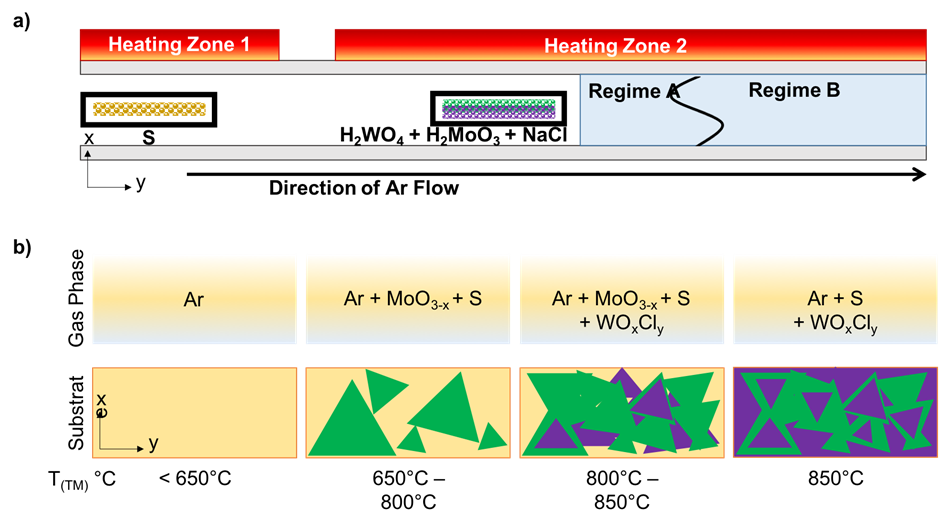
\includegraphics[scale=0.4]{Heterostructures/CVDGrowthSetup.png}
		\caption{CVD furnace setup a) spatial distribution of precursors  b) simplified representation of the growth result (green = Mo region;  purple = W region).}
		\label{fig:HeterostructureCVDGrowthSetup}
	\end{center}
\end{figure}

\begin{figure}[ht]
	\begin{center}
		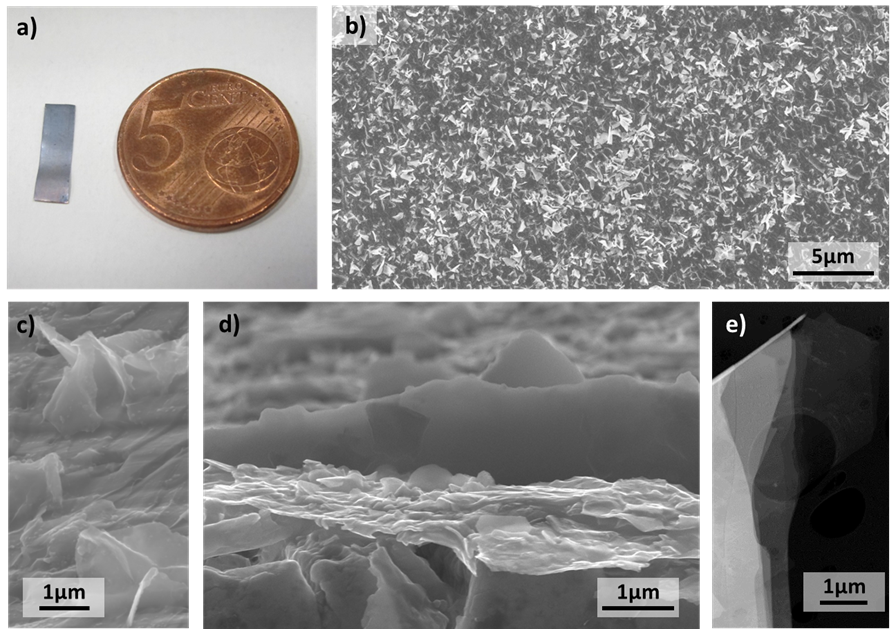
\includegraphics[scale=0.4]{Heterostructures/SEMImages.png}
		\caption{a) $MoS_2/WS_2$ heterobilayer on Au substrate b) SEM image of $MoS_2/WS_2$ heterobilayer on Au substrate c) side; d) cross-sectional SEM image e) STEM image of the flake edge. Adopted from \cite{Sherrell2019}.}
		\label{fig:HeterostructureSEMImages}
	\end{center}
\end{figure}

It is especially easy to achieve vertical growth on Au substrate due to high capture rate of sulphur at the nucleation stage \cite{Gao2015}. This results in good adhesion of the flakes parallel to the surface and high surface area caused by the vertical growths. Relatively big flakes can still be grown using this procedure (Figure \ref{fig:HeterostructureSEMImages}.

\section{Results}

A $WS_2$/$MoS_2$ heterobilayer has been prepared by one step growth CVD a seen in Figure \ref{fig:HeterostructureCVDGrowthSetup}. The heterobilayer has been grown on $SiO_2/Si$ using parameters developed for monolayer growth. The $S$ precursor was placed in one crucible and placed about 20 cm upstream from the growth substrate. The $W$ and $Mo$ precursors, $H_2WO_4$ and $MoO_3$ respectively, were placed in a separate crucible which was located in direct contact with the substrate. The $S$ precursor was then heated up to 150 {\degree}C while the $W$ and $Mo$ are heated up to 850 {\degree}C. The growth is performed in small vacuum with Ar flow. An optical micrograph of a select area of the sample can be seen in Figure \ref{fig:HeterostructureOMSi}. The sample contains large areas of monolayer and bilayer TMDCs with some very small flake of bulk material. Overall the material coverage is quite high.

The sample was then characterised using Raman and PL spectroscopy. A measurement of Raman spectrum was taken from heterobilayer and as seen in Figure \ref{fig:HeterostructureRamanSpectrum} a distinct spectrum of $WS_2$ and $MoS_2$ can be distinguished. The Raman peak positions are 350.1 $cm^{-1}$, 382 $cm^{-1}$, 408.3 $cm^{-1}$ and 417.7 $cm^{-1}$ which can ascribed to $WS_2$ $E^1_{2g}$, $MoS_2$ $E^1_{2g}$, $MoS_2$ $A_{1g}$ and $WS_2$ $A_{1g}$ respectively. Those peak positions correspond to multi layers of the individual materials which indicates a certain level of interaction between the layers.

\begin{figure}[H]
	\begin{center}
		\includegraphics[scale=0.5]{Heterostructures/OmSi.png}
		\caption{Optical micrograph of $WS_2/MoS_2$ heterobilayer on $SiO_2/Si$}
		\label{fig:HeterostructureOMSi}
	\end{center}
\end{figure}

\begin{figure}[H]
	\begin{center}
		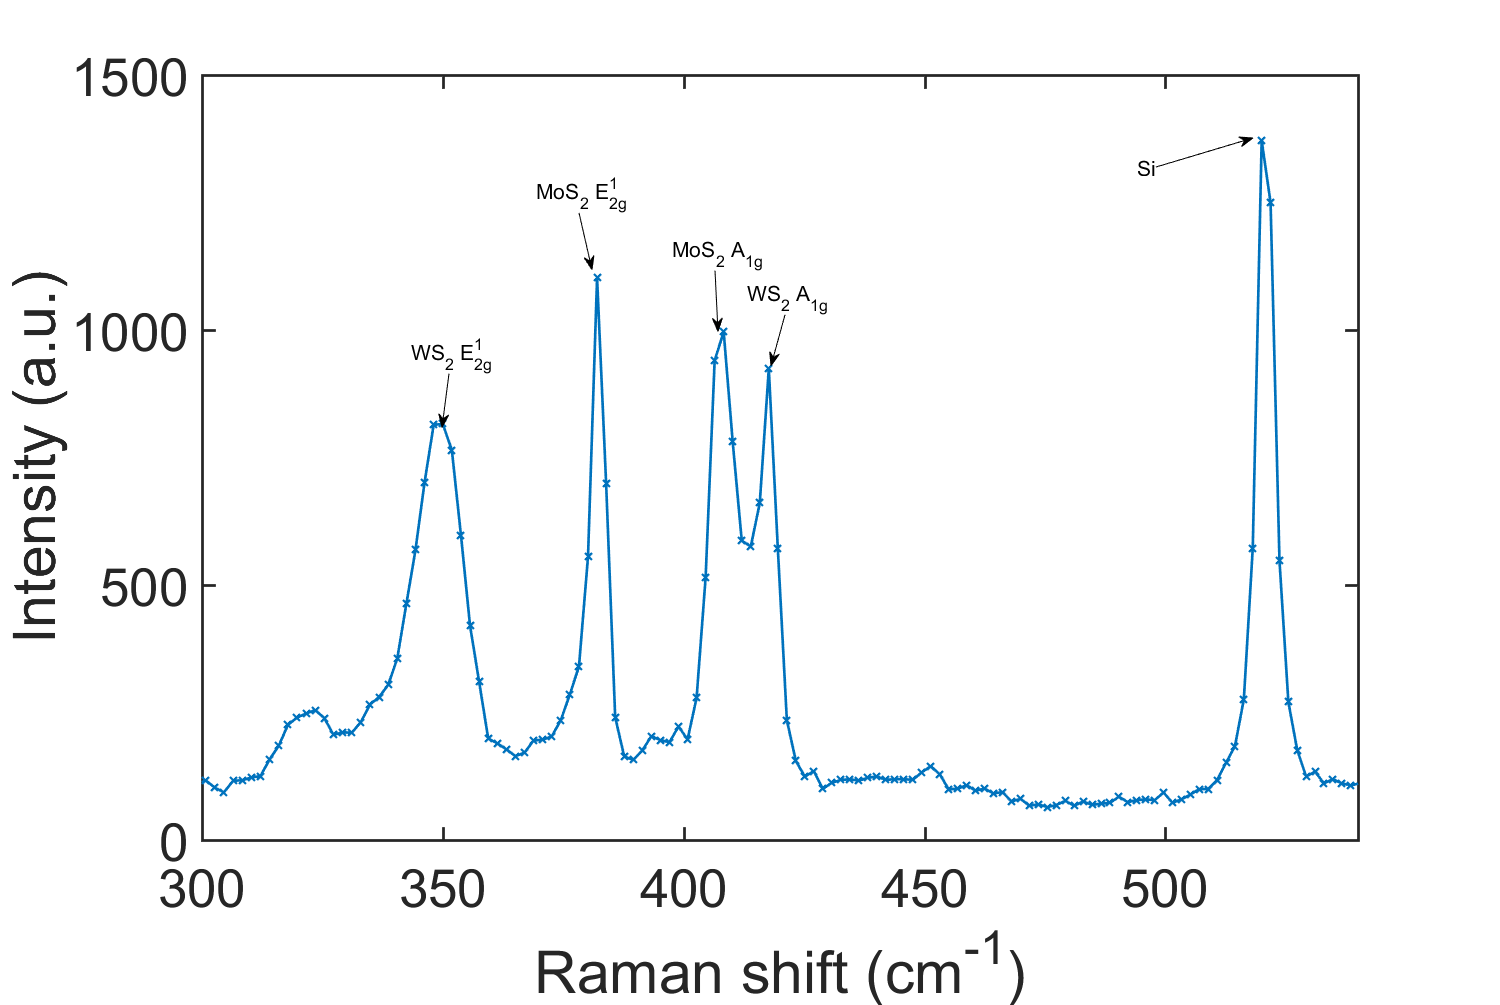
\includegraphics[scale=0.3]{Heterostructures/RamanSpectrum2.png}
		\caption{Raman spectrum of $WS_2$/$MoS_2$ heterobilayer}
		\label{fig:HeterostructureRamanSpectrum}
	\end{center}
\end{figure}

There is a monolayer and bilayer $MoS_2$ found around the heterobilayer area with no $WS_2$ grown  indicating that the $WS_2$ flake has grown on top of the $MoS_2$ layer. The area surrounding the heterobilayer shows a spectrum as seen in Figure \ref{fig:HeterostructuresRamanSpectraMonoBi}. 

\begin{figure}[H]
	\begin{center}
		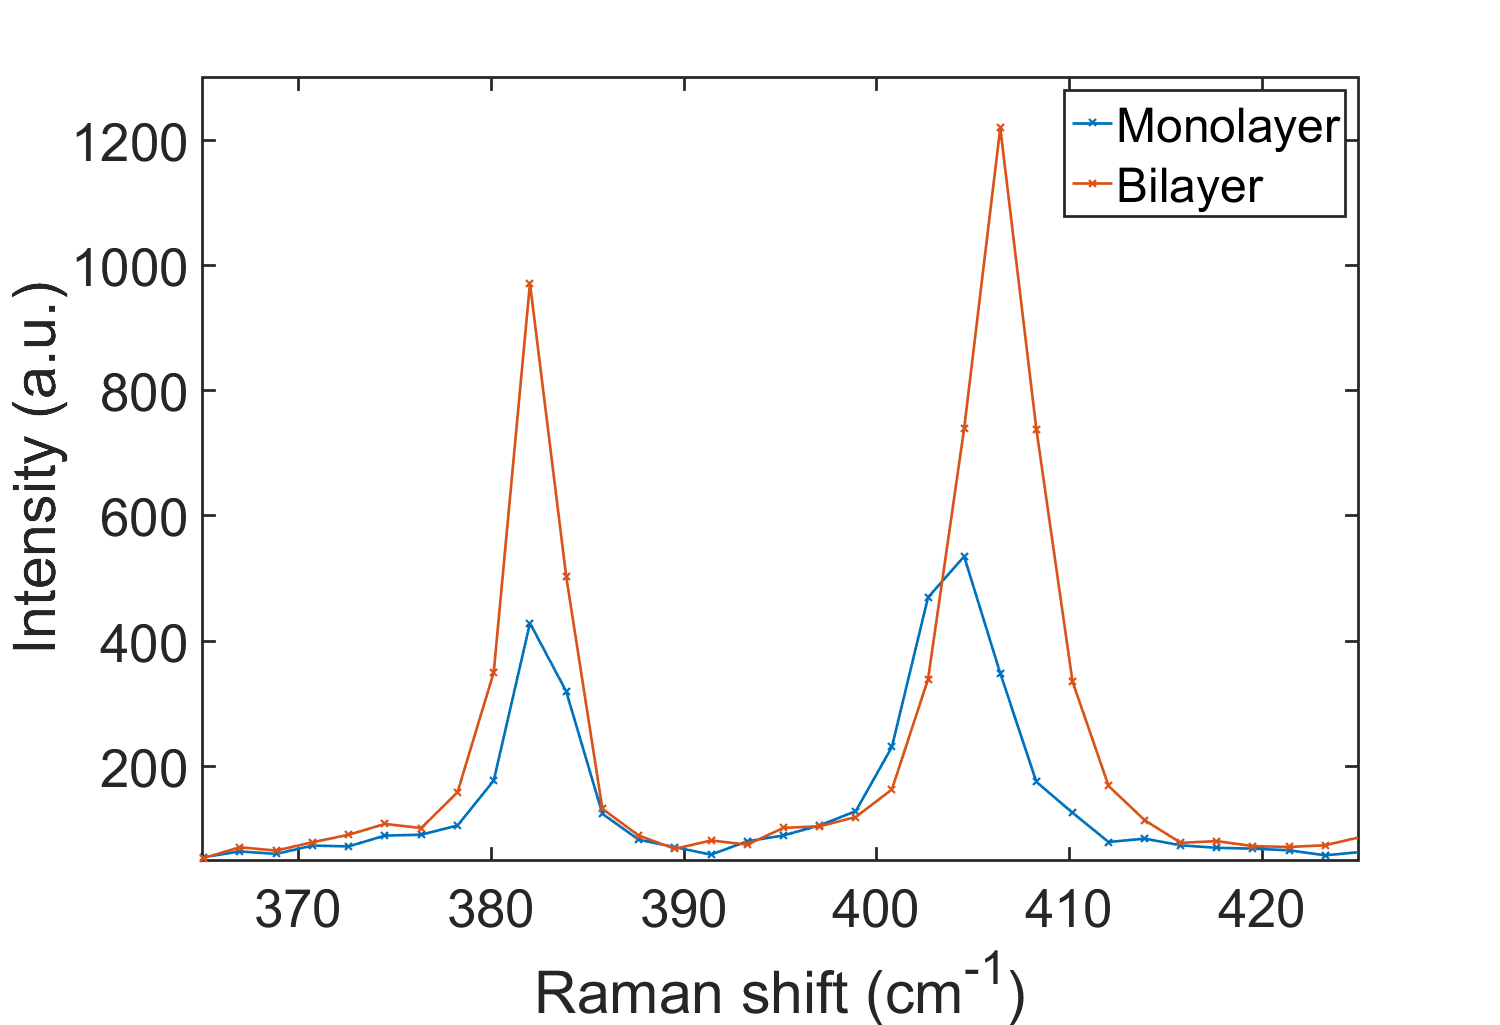
\includegraphics[scale=0.3]{Heterostructures/RamanSpectraMonoBi2.png}
		\caption{Raman spectra of mono and bilayer $MoS_2$}
		\label{fig:HeterostructuresRamanSpectraMonoBi}
	\end{center}
\end{figure}

The positions of the peaks are 382.7 $cm^{-1}$ and 404 $cm^{-1}$ for the monolayer and 382.4 $cm^{-1}$ and 406.4 $cm^{-1}$ for the bilayer. 

It has been shown that in $WMoSe_2$ alloy as more of the alloying metal is added the characterstic Raman peaks ($E^1_{2g}$ and $A_{1g}$) of the primary structure become less intense and shifted \cite{Zhang2014}. Due to presence of both $WS_2$ and $MoS_2$ characteristic peaks at relatively high intensity as well as lack of significant shift in the observed peak position it can be concluded that the sample is not a complete alloy. Similarly the PL in TMDC alloy, like $MoWSe_2$, shows the main A peak shifting from position of the PL peak in monolayer of one of the TMDC to the other \cite{Wang2015}. As seen in Figure \ref{fig:HeterostructuresPLSpectrumFitted} both of the peaks from $WS_2$ as well as $Mo_2$. It further indicates that the material is not mostly an alloy and includes pure monolayers of $WS_2$ and $MoS_2$. It is possible that each of the monolayer in the heterobilayer is alloyed to a small degree but further studies are necessary to properly quantify these results.

The sample was then mapped using Raman spectroscopy. As seen in Figure \ref{fig:HeterostructuresRamanIntensityE} the intensity of $E^1_{2g}$ peak varies across the mapped area for both $WS_2$ and $MoS_2$. The more intense areas indicate more layers of $WS_2$ which is placed on top of $MoS_2$. Where the intensity of $WS_2$ $E^1_{2g}$ peak is higher and therefore there is more layers of $WS_2$ the intensity of $MoS_2$ $E^1_{2g}$ is reduced. 

\begin{figure}[H]
	\begin{center}
		\begin{subfigure}[b]{0.45\textwidth}
			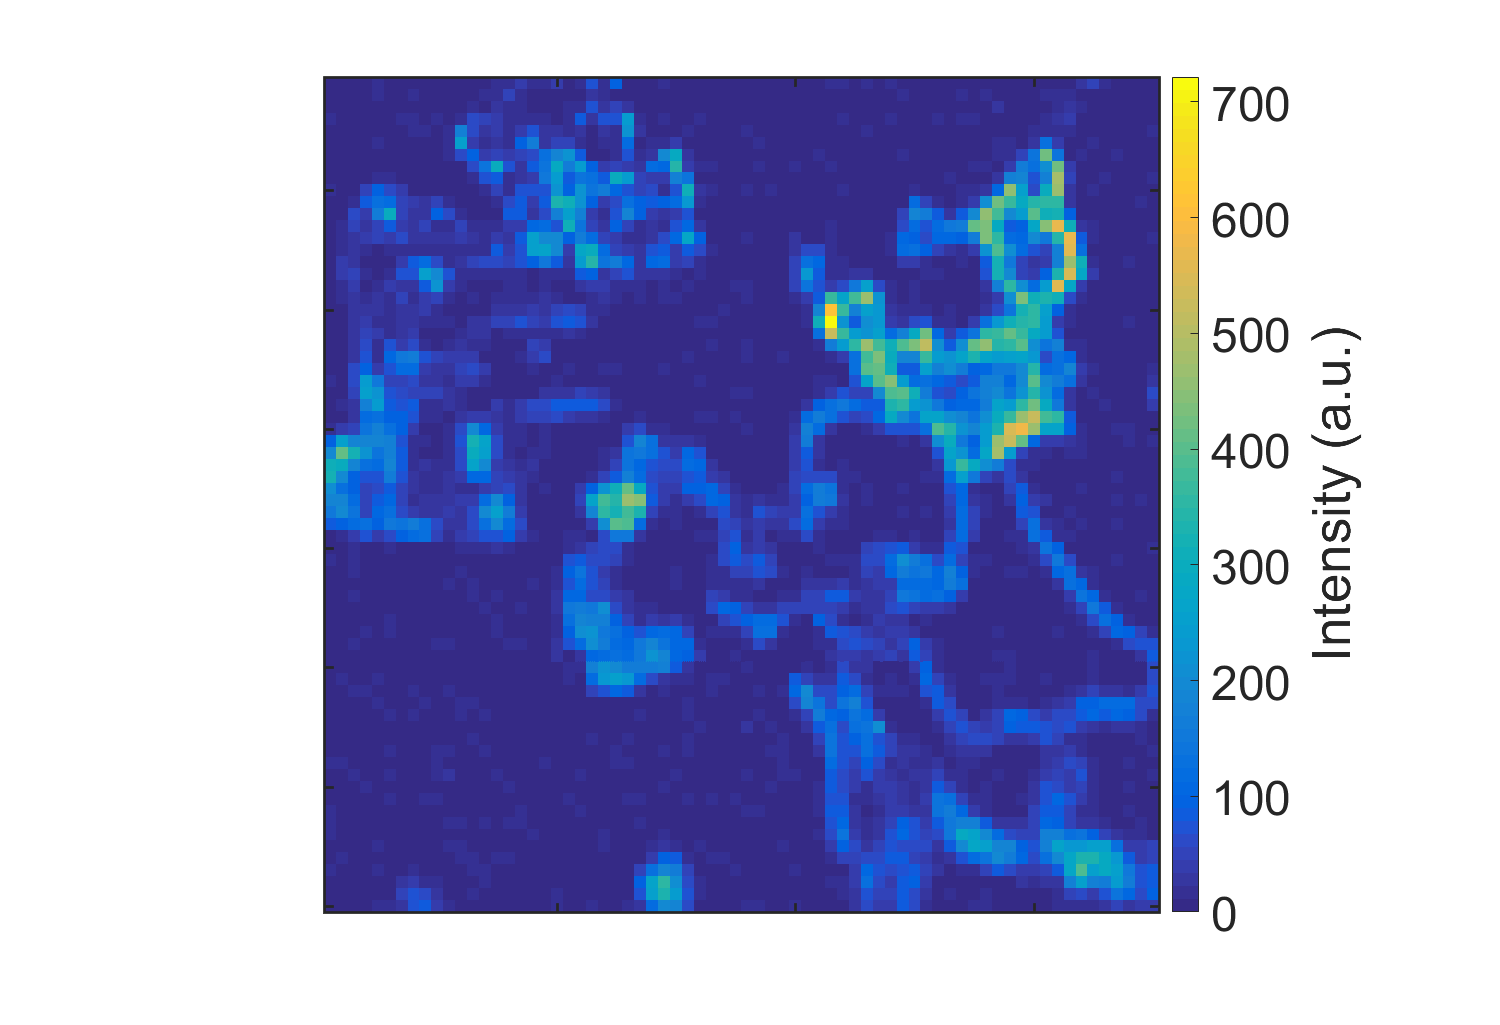
\includegraphics[width=\textwidth]{Heterostructures/RamanIntensityMapEWS2.png}
			\caption{$WS_2$}
			\label{fig:HeterostructuresRamanIntensityEWS2}
		\end{subfigure}
		\begin{subfigure}[b]{0.45\textwidth}
			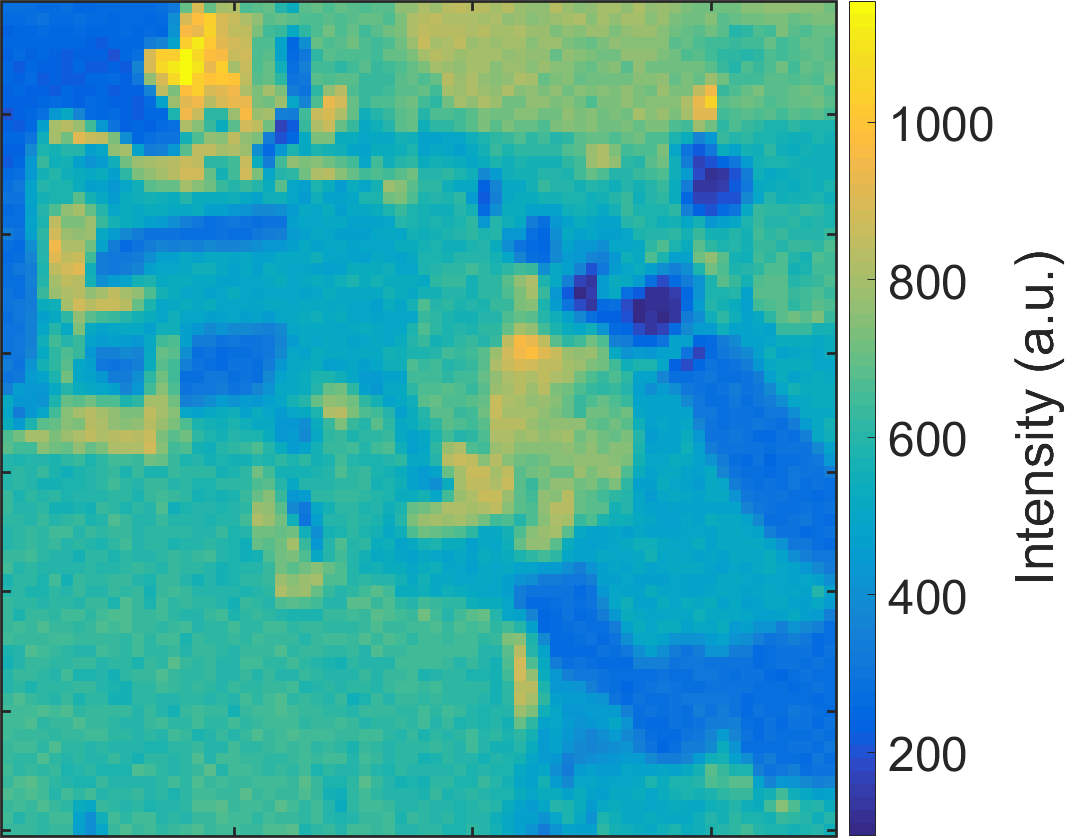
\includegraphics[width=\textwidth]{Heterostructures/RamanIntensityMapEMoS2.png}
			\caption{$MoS_2$}
			\label{fig:HeterostructuresRamanIntensityEMoS2}
		\end{subfigure}
		\caption{Map of Raman $E^1_{2g}$ peak intensity}
		\label{fig:HeterostructuresRamanIntensityE}
	\end{center}
\end{figure}

\begin{figure}[H]
	\begin{center}
		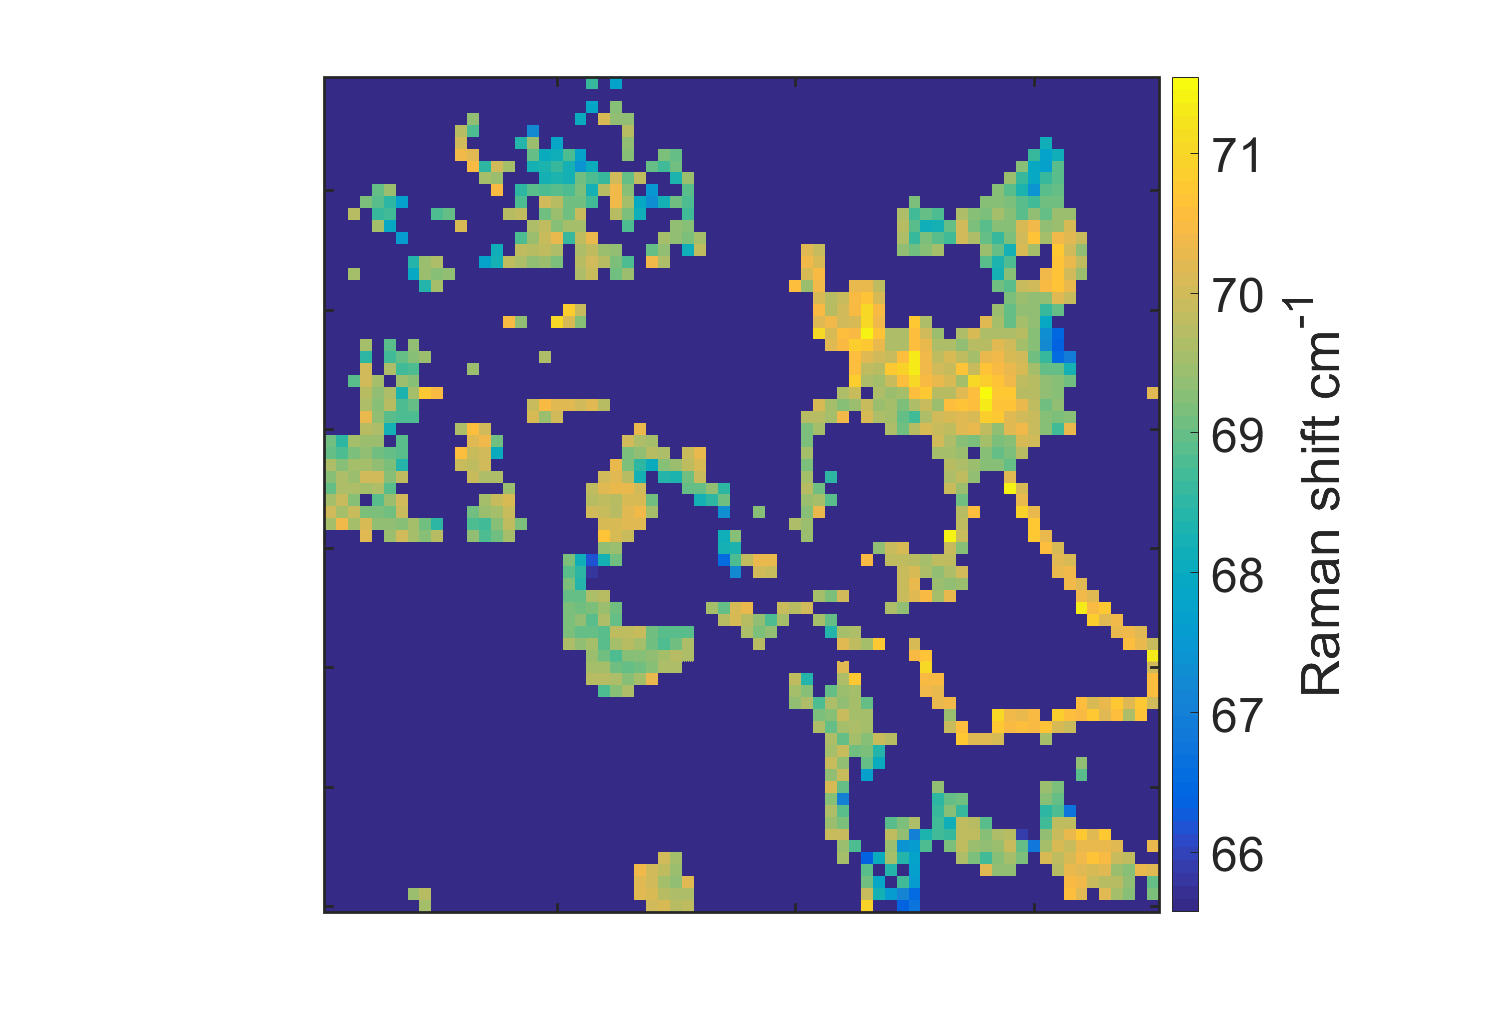
\includegraphics[scale=0.3]{Heterostructures/HeterostructureRamanDifferenceW.png}
		\caption{Difference between $WS_2$ $A_{1g}$ and $E^1_{2g}$ peak position}
		\label{fig:HeterostructuresRamanDifferenceW}
	\end{center}
\end{figure}

To better estimate the number of layers the difference between $A_{1g}$ and $E^1_{2g}$ peak positions has been also calculated as seen in Figure \ref{fig:HeterostructuresRamanDifferenceW}. By excluding the bulk flakes and leaving the flakes with less or equal to 3 layers of $WS_2$ it can estimated that about 25\% of the area is covered with $WS_2/MoS_2$ heterobilayer.

\begin{figure}[H]
	\begin{center}
		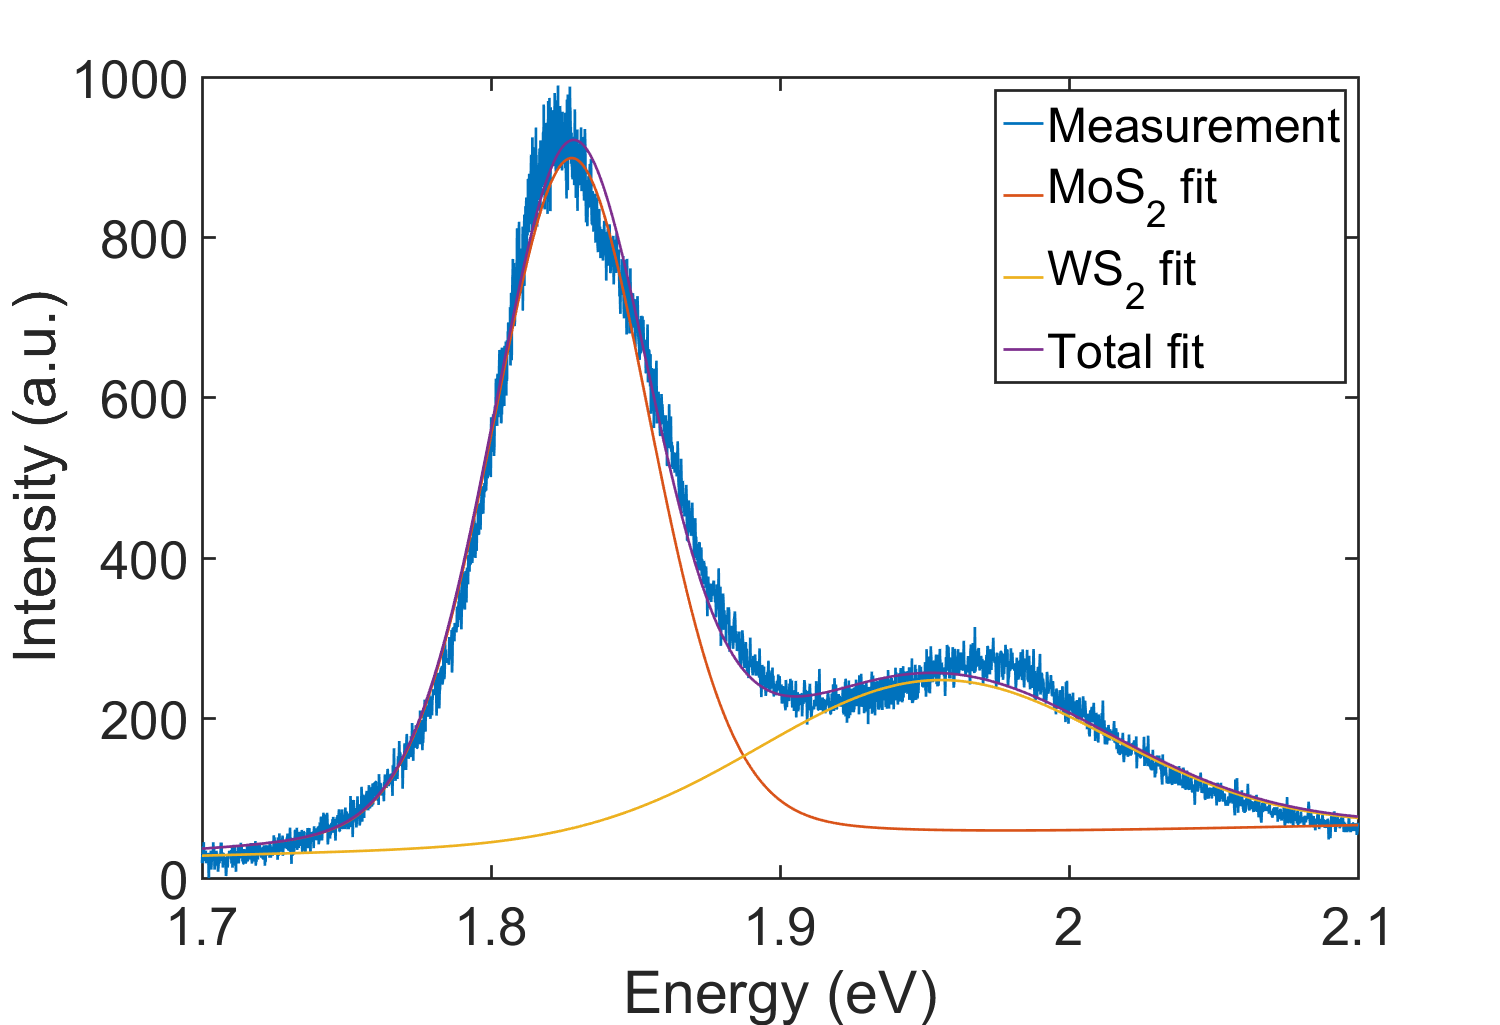
\includegraphics[scale=0.3]{Heterostructures/HeterostructurePLSpectrumFitted.png}
		\caption{PL spectrum of $MoS_2/WS_2$ heterobilayer}
		\label{fig:HeterostructuresPLSpectrumFitted}
	\end{center}
\end{figure}

The PL spectrum of heterobilayer can be seen in Figure \ref{fig:HeterostructuresPLSpectrumFitted}. There are two distinct peaks, one  at 1.824 eV and second at 1.971 eV. The position of the $MoS_2$ PL peak is consistent with the position of the monolayer $MoS_2$ as seen in Figure \ref{fig:HeterostructuresPLSpectrumMono} which is 1.825 eV. Those PL peaks from heterobilayer therefore correspond to both $MoS_2$ and $WS_2$ monolayers indicating that the spectrum is additive. The $MoS_2$ peak is also much stronger than $WS_2$ despite the fact that isolated monolayer of $WS_2$ shows much stronger PL than a monolayer of $MoS_2$. The $MoS_2$ peak has a FWHM of 65.47 meV while the $WS_2$ PL peak has a FWHM of 142.4 meV. 

\begin{figure}[H]
	\begin{center}
		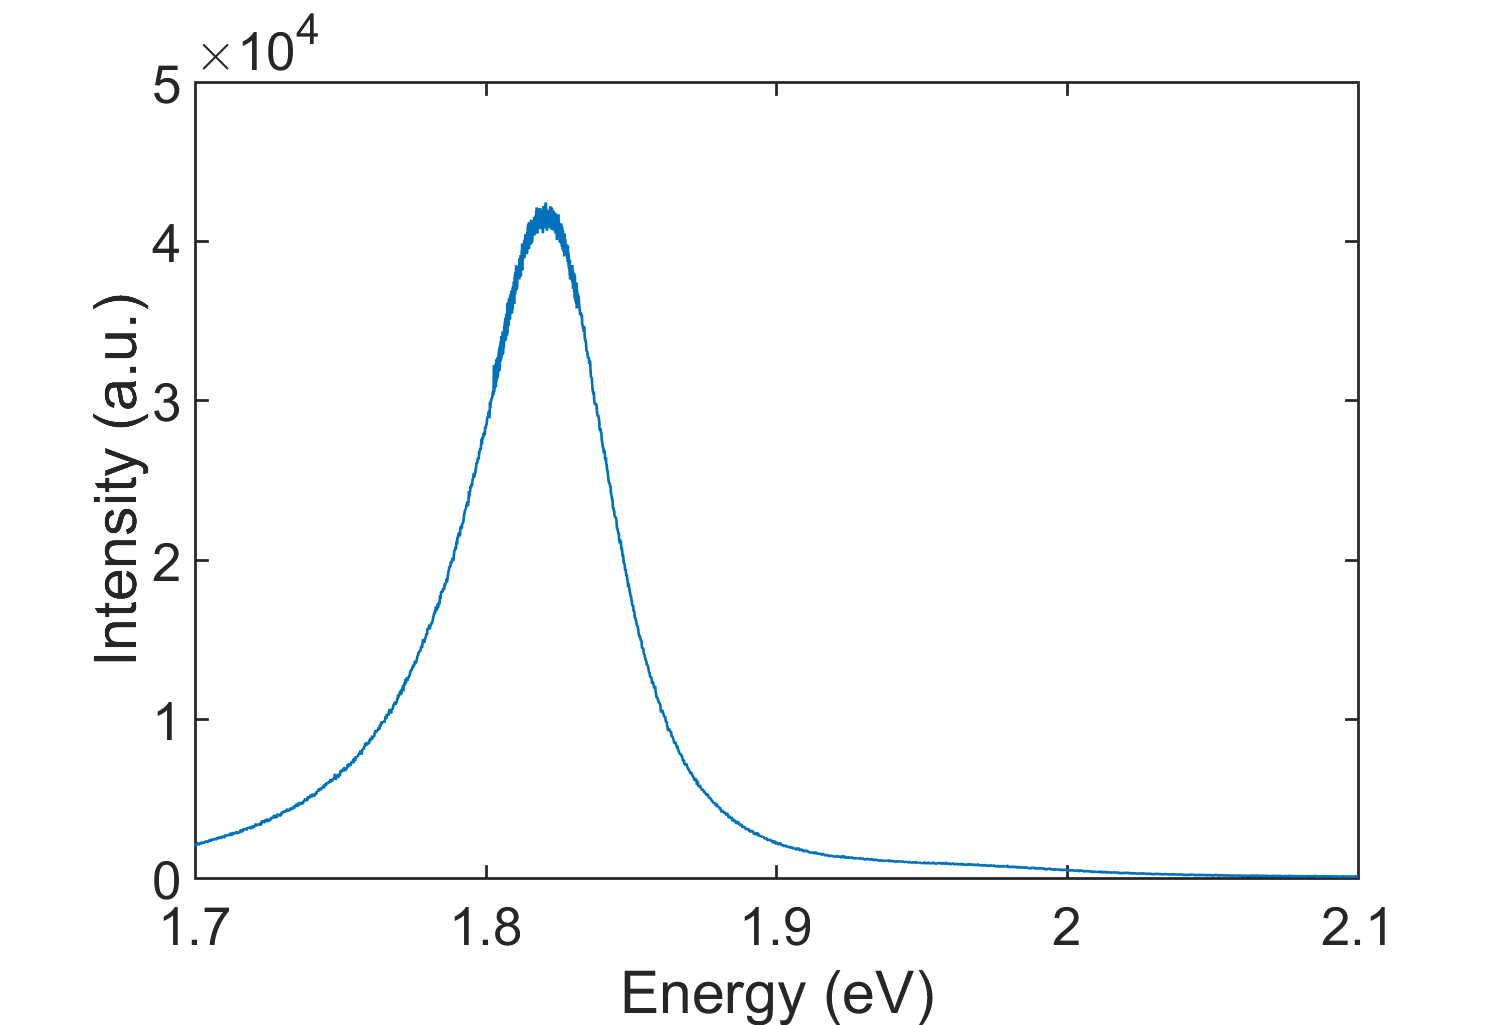
\includegraphics[scale=0.3]{Heterostructures/HeterostructurePLSpectrumMono.png}
		\caption{PL spectrum of $MoS_2$ monolayer}
		\label{fig:HeterostructuresPLSpectrumMono}
	\end{center}
\end{figure}

The sample was also mapped using PL spectroscopy as seen in Figure \ref{fig:HeterostructuresPLIntensityMap11}. The most intense PL can be observed in areas of monolayer $MoS_2$ and much weaker everywhere else. The position map of PL peaks from both $MoS_2$ and $WS_2$ can be seen further in Figure \ref{fig:HeterostructuresPLPositionsMap}. Most of the PL of $MoS_2$ is centred around 1.82 eV with smaller part ($\sim 8 \%$) centred around 1.802 eV. It seems therefore that majority of the $MoS_2$ is a monolayer $MoS_2$ while the PL peaks at 1.802 eV indicate a $MoS_2$ bilayer. The $WS_2$ PL position map reveals most of the PL peaks centred around 1.965 eV and smaller part ($\sim 16 \%$) centred around 1.935 eV. Similarly to $MoS_2$ the majority of the $WS_2$ is therefore monolayer with small part of it being bilayer $WS_2$.

\begin{figure}[H]
	\begin{center}
		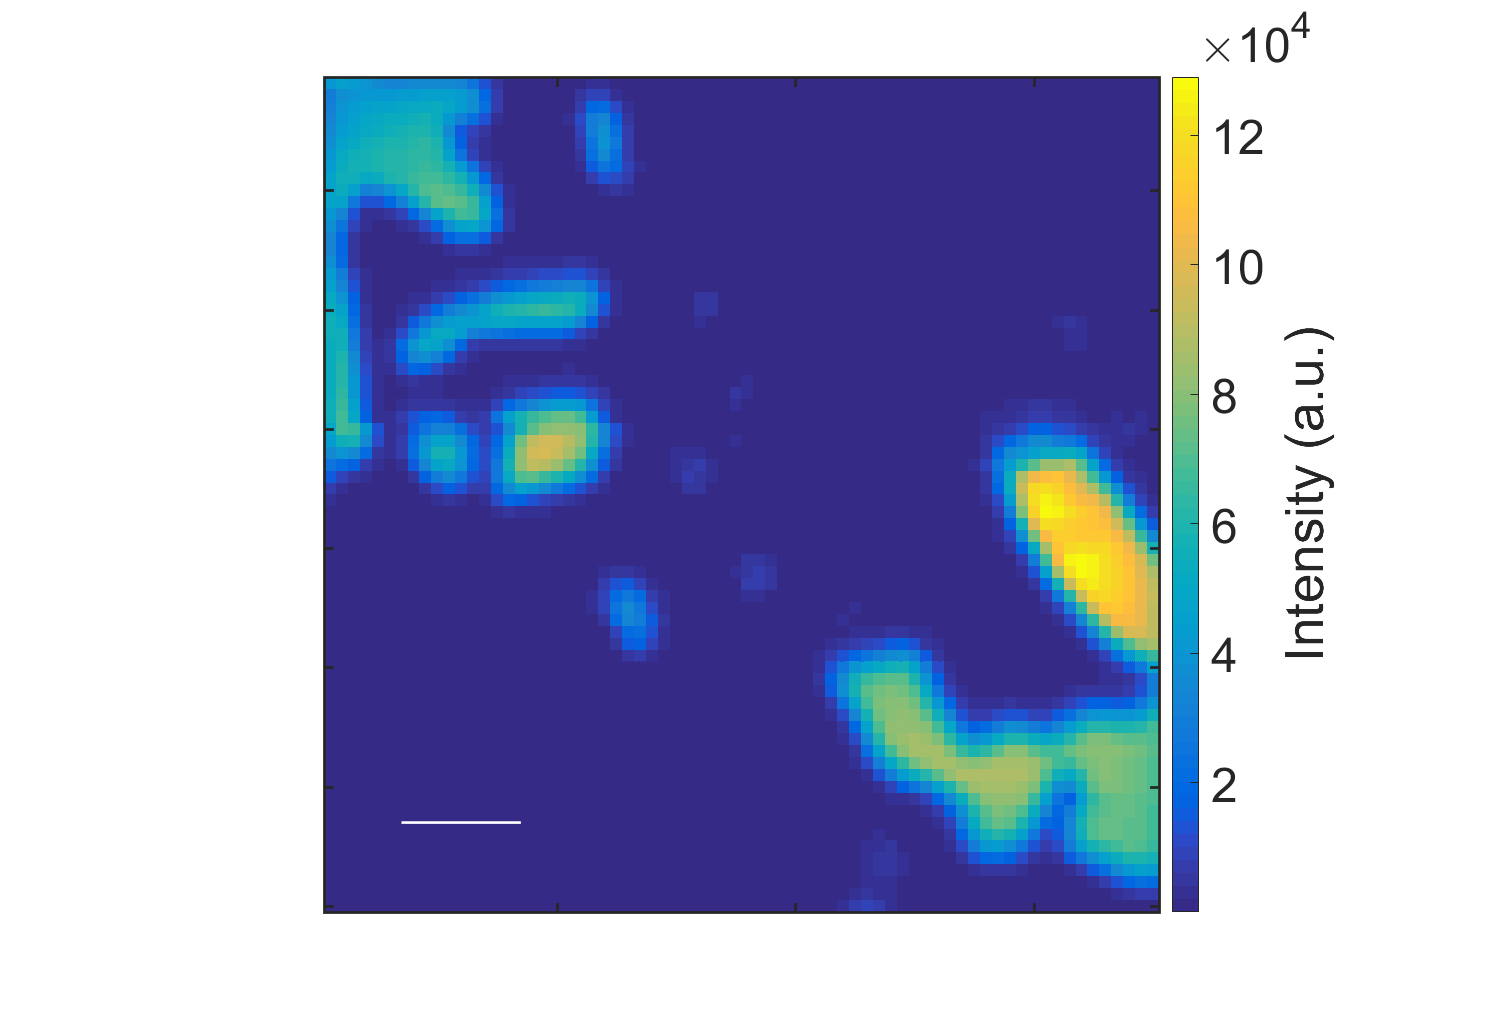
\includegraphics[scale=0.3]{Heterostructures/PLIntensityMap11.png}
		\caption{Integrated PL intensity map. Scalebar is 10$\mu m$.}
		\label{fig:HeterostructuresPLIntensityMap11}
	\end{center}
\end{figure}

\begin{figure}[H]
	\begin{center}
		\begin{subfigure}[b]{0.5\textwidth}
			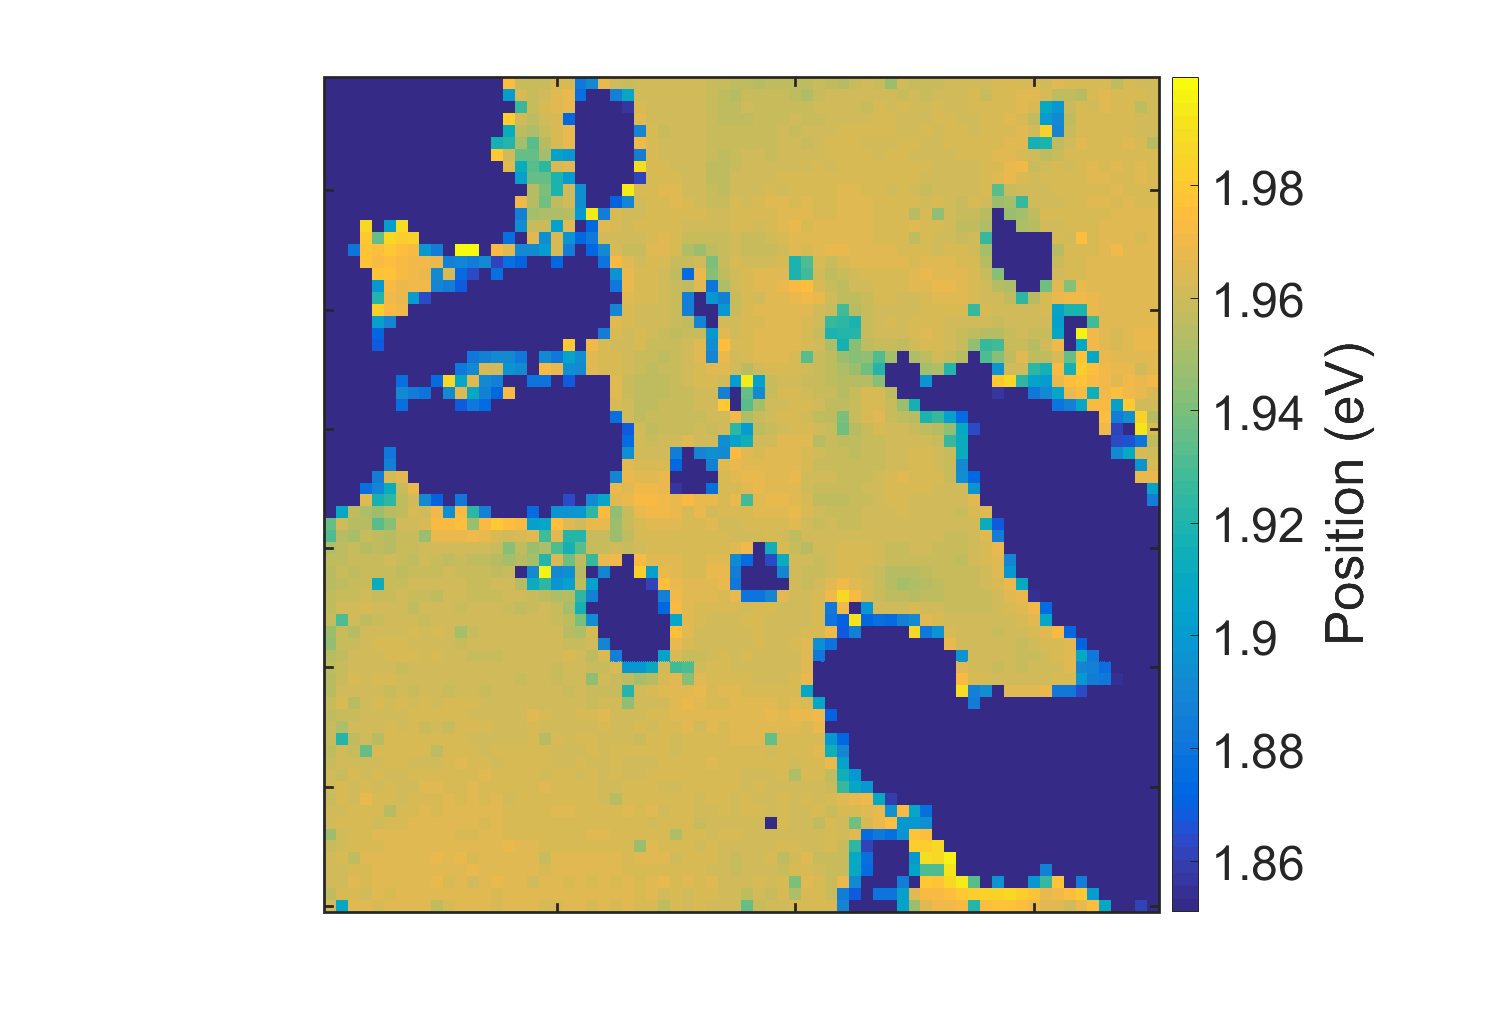
\includegraphics[scale=0.25]{Heterostructures/PLPositionMap21.png}
			\caption{PL position of the $MoS_2$ flake.}
			\label{fig:HeterostructuresPLPosition21Map}
		\end{subfigure}
		\begin{subfigure}[b]{0.45\textwidth}
			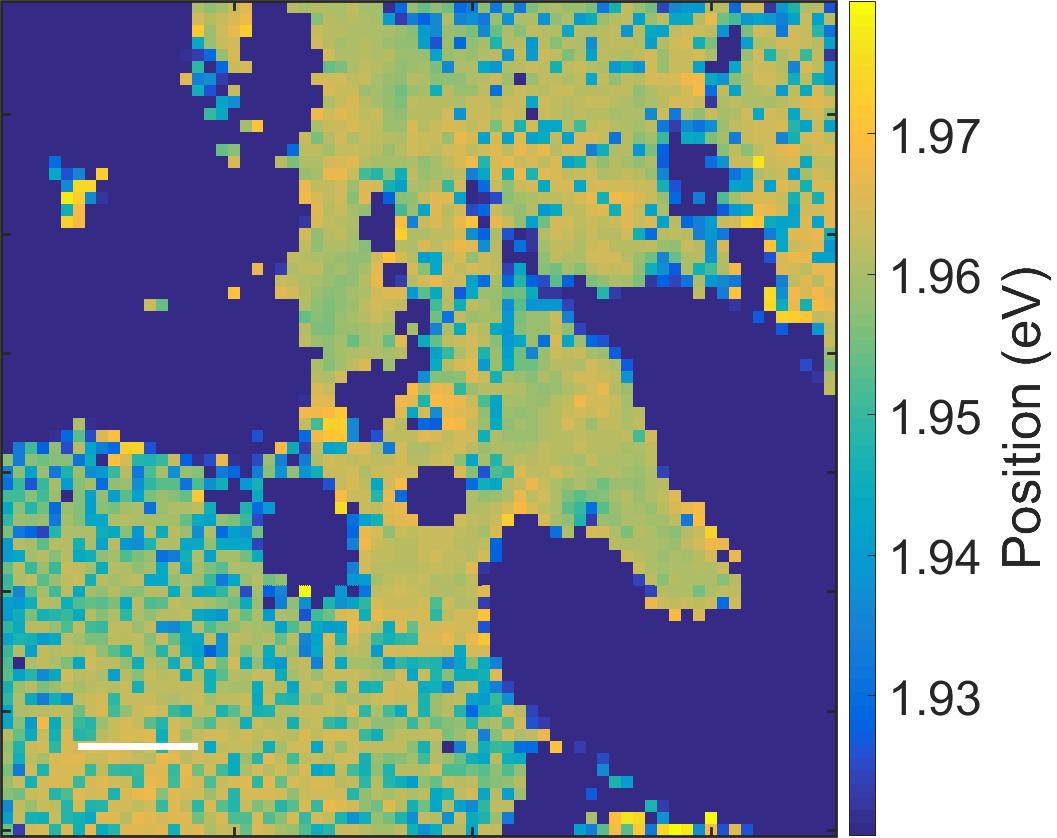
\includegraphics[scale=0.25]{Heterostructures/PLPositionMap22.png}
		\caption{PL position of the $WS_2$ flake.}
		\label{fig:HeterostructuresPLPosition22Map}
		\end{subfigure}
		\caption{Map of PL peak positions. Scalebar is 10$\mu m$.}
		\label{fig:HeterostructuresPLPositionsMap}
	\end{center}
\end{figure}

The similar growth procedure was then used to grow $WS_2/MoS_2$ heterobilayer on a gold substrate. As seen in Figure \ref{fig:HeterostructuresOMAu} the material coverage of the substrate is complete. The material also seems to be thick with irregular, rough surface. There are no visible triangles or continuous layers like seen in a $SiO_2/Si$ substrate. This is most likely due to vertical growth which can occur on gold substrate as opposed to $SiO_2/Si$ substrate.

\begin{figure}[H]
	\begin{center}
		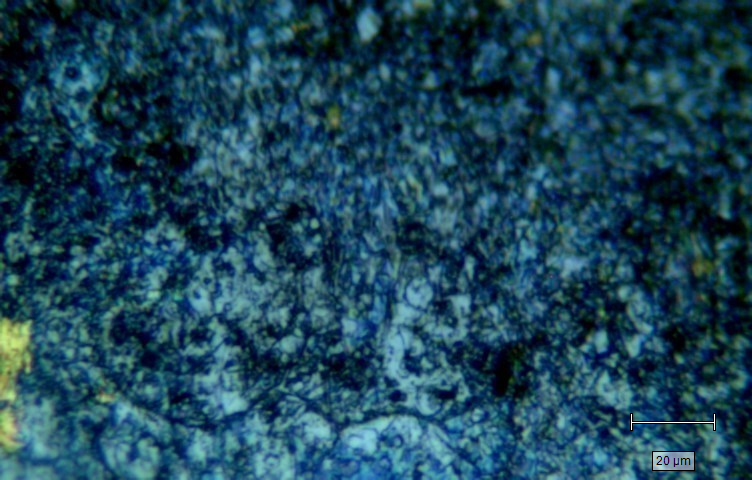
\includegraphics[scale=0.3]{Heterostructures/OMAu.png}
		\caption{Opitcal micrograph of the $WS_2/MoS_2$ on Au substrate}
		\label{fig:HeterostructuresOMAu}
	\end{center}
\end{figure}

The sample was then mapped using Raman spectroscopy. As seen in Figure \ref{fig:HeterostructuresRamanSpectrumAu} the $WS_2$ and $MoS_2$ Raman peaks $E^1_{2g}$ and $A_{1g}$ can be identified.

\begin{figure}[H]
	\begin{center}
		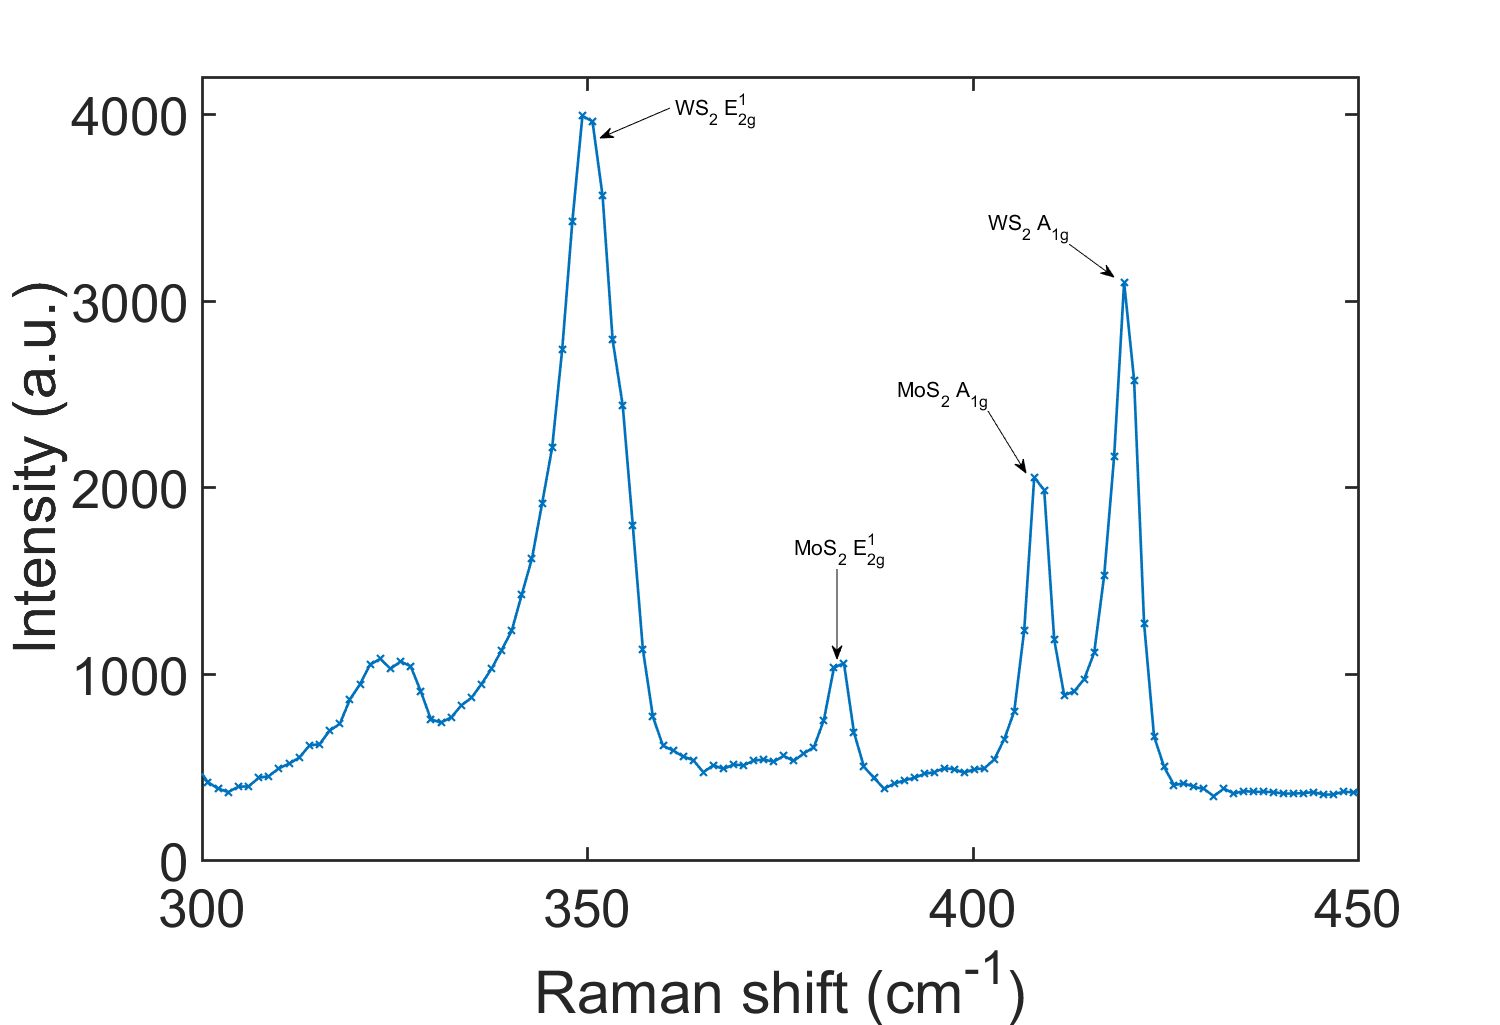
\includegraphics[scale=0.3]{Heterostructures/RamanSpectrumAu.png}
		\caption{Raman spectrum of $WS_2/MoS_2$ on Au substrate}
		\label{fig:HeterostructuresRamanSpectrumAu}
	\end{center}
\end{figure}

As seen in Figure \ref{fig:HeterostructuresRamanIntensityEMaps} the $MoS_2$ $E^1_{2g}$ can be seen across the entire scanned area. On the other the $WS_2$ $E^1_{2g}$ peak can be seen less spread around. Additionally the areas with high intensity $WS_2$ $E^1_{2g}$ coincide with low intensity $MoS_2$ $E^1_{2g}$. It implies therefore that similarly to the $SiO_2/Si$ substrate the $WS_2$ grows on top of the $MoS_2$ which results in a weaker Raman signal from $MoS_2$ from areas where thick $WS_2$ has grown on top of the underlying $MoS_2$. 

\begin{figure}[H]
	\begin{center}
		\begin{subfigure}[b]{0.5\textwidth}
			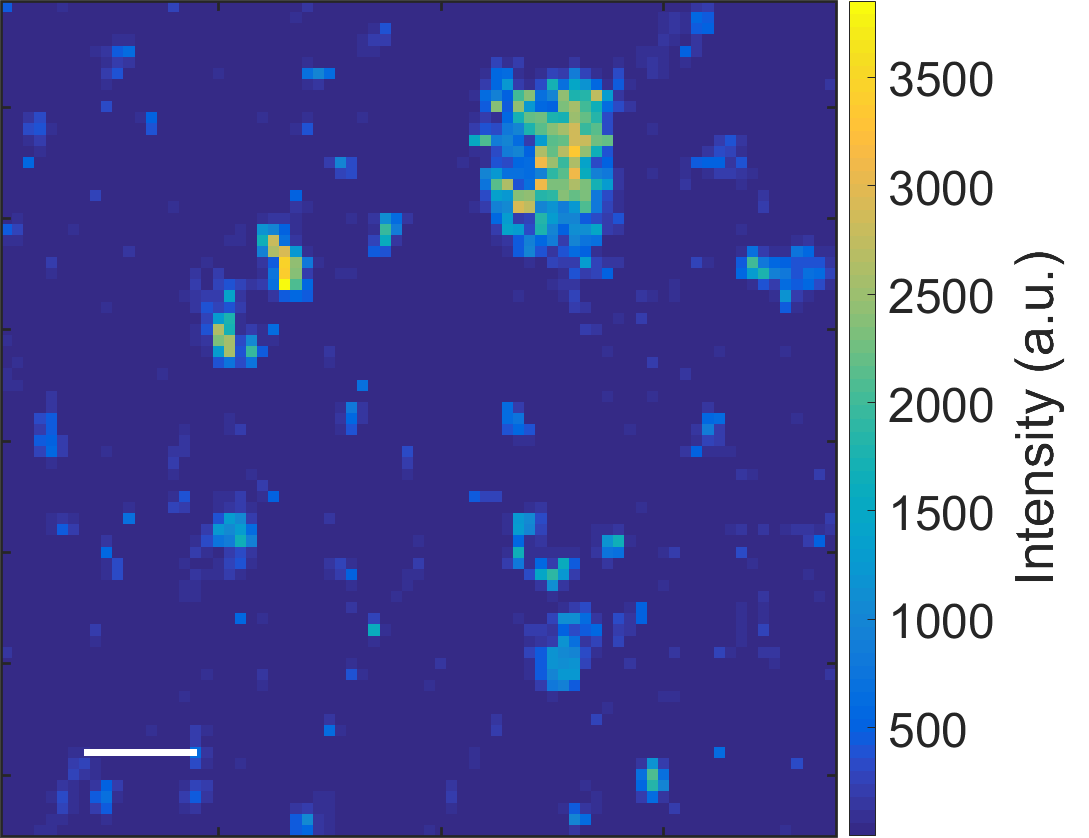
\includegraphics[scale=0.25]{Heterostructures/HeterostructuresRamanIntensityEWAu.png}
			\caption{$WS_2$}
			\label{fig:HeterostructuresRamanIntensityEWAu}
		\end{subfigure}
		\begin{subfigure}[b]{0.45\textwidth}
			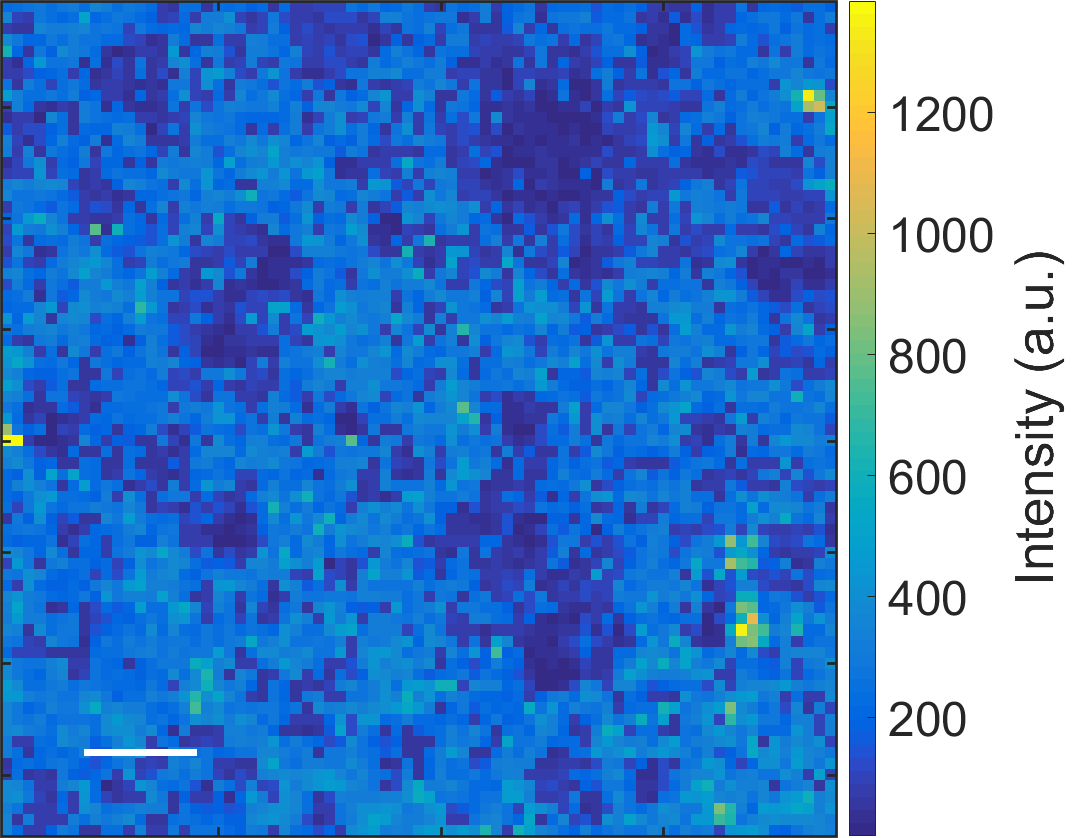
\includegraphics[scale=0.25]{Heterostructures/HeterostructuresRamanIntensityEMoAu.png}
			\caption{$MoS_2$}
			\label{fig:HeterostructuresRamanIntensityEMoAu}
		\end{subfigure}
		\caption{Raman $E^1_{2g}$ intensity maps. Scalebar is 10$\mu m$.}
		\label{fig:HeterostructuresRamanIntensityEMaps}
	\end{center}
\end{figure}

The peaks positions for $WS_2$ are on average 349.1 $cm^{-1}$ and 418.5 $cm^{-1}$ for $E^1_{2g}$ and $A_{1g}$ respectively. Similarly for $MoS_2$ the peaks positions are 382.5 $cm^{-1}$ and 408.6 $cm^{-1}$ for $E^1_{2g}$ and $A_{1g}$ respectively. This indicates that both $MoS_2$ and $WS_2$ are mostly few layers thick. It can be estimated that in the measured area the $WS_2$ coverage and therefore the $WS_2$/$MoS_2$ heterobilayer presence is at least 8{\%}.

Due to the gold substrate the PL is partially quenched which combined with weak PL signal coming from few layer $WS_2$ and $MoS_2$ makes it difficult to make any meaningful measurement.

Compared to previously reported work on TMDCs, the performance in both hydrogen evolution ($\sim$0.1 \% IPCE) and water oxidation ($\sim$0.1 \% IPCE) is improved \cite{Fu2015}. Further data and analysis of the photoelectrocatalytical performance of this heterobilayer has been reported in \cite{Sherrell2019}.

\section{Conclusion}

The $MoS_2/WS_2$ heterobilayer has successfully been grown on $SiO_2/Si$ as well Au substrates. Their structure has been then successfully assessed with the help of PL and Raman spectroscopy. Raman and PL maps revealed that at least 8\% of the investigated areas has been covered in heterobilayers. Their performance as an photoelectrocatalyst for water oxydation and hydrogen evolution has been further evaluated and found to be superior to the previously reported values. Overall those promising results warrant further research and development of one step growth to achieve better heterobilayer coverage and performance.